\documentclass[a4paper]{article}
\usepackage[spanish]{babel}
\usepackage[utf8]{inputenc}
\usepackage{graphicx}
\usepackage{enumerate}
\usepackage{listings}
\usepackage{color}
\usepackage{indentfirst}
\usepackage{fancyhdr}
\usepackage{latexsym}
\usepackage[colorlinks=true, linkcolor=black]{hyperref}
%\usepackage{makeidx}
%\usepackage{float}
\usepackage{calc}
\usepackage{amsmath, amsthm, amssymb}
\usepackage{amsfonts}
%\lstset{language=C}
\definecolor{gray}{gray}{0.5}
\definecolor{light-gray}{gray}{0.95}
\definecolor{orange}{rgb}{1,0.5,0}

\usepackage{fancyhdr}
\pagestyle{fancy}

%\renewcommand{\chaptermark}[1]{\markboth{#1}{}}
\renewcommand{\sectionmark}[1]{\markright{\thesection\ - #1}}

\fancyhf{}

\fancyhead[LO]{Sección \rightmark} % \thesection\ 
\fancyfoot[LO]{\small{Arístides Catalano, Laura Muiño, Jorge Quintana}}
\fancyfoot[RO]{\thepage}
\renewcommand{\headrulewidth}{0.5pt}
\renewcommand{\footrulewidth}{0.5pt}
\setlength{\hoffset}{-0.8in}
\setlength{\textwidth}{16cm}
%\setlength{\hoffset}{-1.1cm}
%\setlength{\textwidth}{16cm}
\setlength{\headsep}{0.5cm}
\setlength{\textheight}{25cm}
\setlength{\voffset}{-0.7in}
\setlength{\headwidth}{\textwidth}
\setlength{\headheight}{13.1pt}

\renewcommand{\baselinestretch}{1.1}  % line spacing


% \setcounter{secnumdepth}{2}
\usepackage{underscore}
\usepackage{caratula}
\usepackage{url}
\usepackage{float}

\newcommand{\cod}[1]{{\tt #1}}
\newcommand{\negro}[1]{{\bf #1}}
\newcommand{\ital}[1]{{\em #1}}
\newcommand{\may}[1]{{\sc #1}}
\newcommand{\tab}{\hspace*{2em}}

\hypersetup{
 pdfstartview= {FitH \hypercalcbp{\paperheight-\topmargin-1in-\headheight}},
 pdfauthor={Grupo},
 pdfsubject={Dise\~{n}o}
}

\lstdefinestyle{customc}{
  backgroundcolor=\color{light-gray},
  belowcaptionskip=1\baselineskip,
  breaklines=true,
  numbers=left,
  xleftmargin=\parindent,
  language=C,
  showstringspaces=false,
  basicstyle=\footnotesize\ttfamily,
  keywordstyle=\bfseries\color{blue},
  commentstyle=\itshape\color{gray},
  identifierstyle=\color{black},
  stringstyle=\color{orange},
}

\lstdefinestyle{customasm}{
  backgroundcolor=\color{light-gray},
  belowcaptionskip=1\baselineskip,
  numbers=left,
  xleftmargin=\parindent,
  language=[x86masm]Assembler,
  keywordstyle=\bfseries\color{blue},
  basicstyle=\footnotesize\ttfamily,
  commentstyle=\itshape\color{gray},
}

\lstset{escapechar=@}


\begin{document}

\thispagestyle{empty}
\materia{Sistemas Operativos}
\submateria{Segundo Cuatrimestre de 2015}
\titulo{Trabajo Práctico I}
\subtitulo{Scheduling}
\integrante{}{}{}
\integrante{Laura Muiño}{399/11}{mmuino@dc.uba.ar}
\integrante{}{}{}

\makeatletter

\maketitle
\newpage

\thispagestyle{empty}
\vfill

\thispagestyle{empty}
\vspace{3cm}
\tableofcontents
\newpage

\newenvironment{myindentpar}[1]
{\begin{list}{1}
         {\setlength{\leftmargin}{#1}}
         \item[]
}
{\end{list} }

%\normalsize
\newpage

% -------------------------------------------------------
% Introducccion
% -------------------------------------------------------
%\input{intro.tex}
% -------------------------------------------------------
% Ejercicios 1 y 2
% -------------------------------------------------------
%\input{ej1-2/ej1-2.tex}
% -------------------------------------------------------
% Ejercicios 3 y 4
% -------------------------------------------------------
%\newpage
%\input{ej3-4/ej3-4.tex}

% -------------------------------------------------------
% Ejercicio 5
% -------------------------------------------------------
%\newpage
%\subsection{Ejercicio 5}

Implementado el Scheduler Round-Robin, se desea analizar ciertos parámetros de calidad del scheduler comparando los mismos para un quantum de 2, 10 y 50 ciclos.
El lote de tareas para la prueba consiste en el siguiente:

\begin{verbatim}
*3 TaskCPU 50 
*2 TaskConsola 5 3 3
\end{verbatim}

Que especifica tres tareas con uso de CPU durante 50 ciclos y 2 tareas que realizan 5 llamadas bloqueantes con duracion de 3 ciclos cada una.

\begin{figure}[h]
  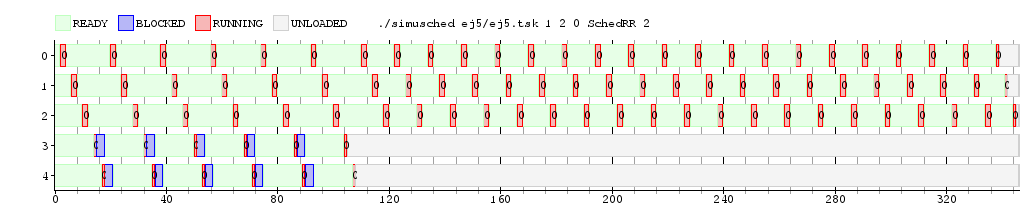
\includegraphics[width=\textwidth]{../ej5/ej5RR1202.png}
  \caption{Tareas ej5 - quantum = 2}
\end{figure}

\begin{figure}[h]
  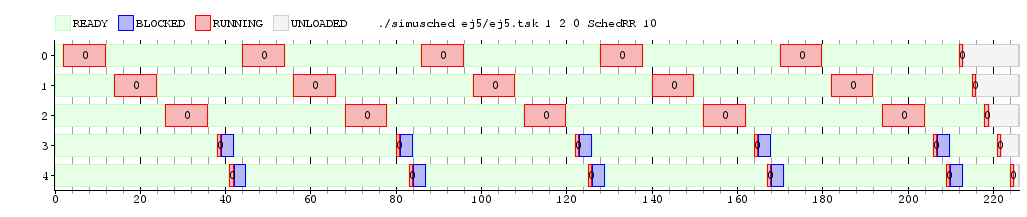
\includegraphics[width=\textwidth]{../ej5/ej5RR12010.png}
  \caption{Tareas ej5 - quantum = 10}
\end{figure}


\begin{figure}[h]
  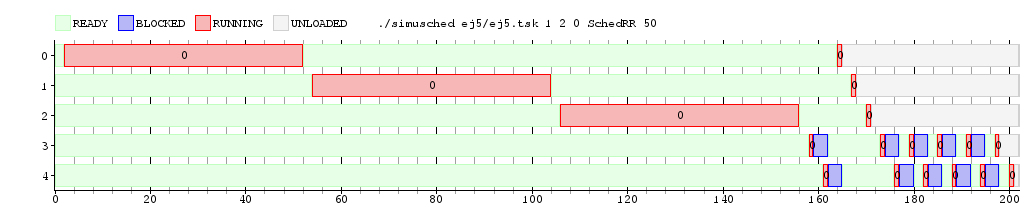
\includegraphics[width=\textwidth]{../ej5/ej5RR12050.png}
  \caption{Tareas ej5 - quantum = 50}
\end{figure}

Los parámetros de calidad a analizar son: latencia, waiting time y tiempo total de ejecución, siendo la latencia el tiempo que la tarea pasa en estado ''listo'' hasta que comienza su ejecución, el waiting time el tiempo que pasa una tarea sin ejecutar desde el momento que está en estado ''listo'' hasta que termina su ejecución, y el tiempo total de ejecución el tiempo que toma la tarea desde que está en estado ''listo'' hasta que cumple con su ejecución.

\begin{table}[h!]
	\begin{center}
		\caption{Parámetros de calidad para el sceduler round robin: SchedRR.}
		\label{tab:table1}
		\begin{tabular}{|l|c|c|c|c|}
			\hline
			& Tarea & Latencia & Waiting time & Tiempo total de ejecución \\
			\hline
			\hline
			& 0 & 2 & & 339 \\ \cline{2-5}
			& 1 & 6 & & 342\\ \cline{2-5}
			Quantum = 2 & 2 & 10 & & 345 \\ \cline{2-5}
			& 3 & 14 & & 105 \\ \cline{2-5}
			& 4 & 17 & & 108 \\ 
			\hline
			\hline
			& 0 & 2 & & 213 \\ \cline{2-5}
			& 1 & 14 & & 216 \\ \cline{2-5}
			Quantum = 10 & 2 & 26 & & 219\\ \cline{2-5}
			& 3 & 38 & & 222 \\ \cline{2-5}
			& 4 & 41 & & 225 \\ 
			\hline
			\hline
			& 0 & 2 & & 165 \\ \cline{2-5}
			& 1 & 54 & & 168 \\ \cline{2-5}
			Quantum = 50 & 2 & 171 & & 156 \\ \cline{2-5}
			& 3 & 158 & & 198 \\ \cline{2-5}
			& 4 & 161 & & 201 \\
			\hline
		\end{tabular}
	\end{center}
\end{table}

\newpage

% -------------------------------------------------------
% Ejercicio 6
% -------------------------------------------------------

% -------------------------------------------------------
% Ejercicio 7
% -------------------------------------------------------
%\newpage
\subsection{Ejecicio 7}

En este ejercicio se pide estudiar el comportamiento del scheduler Mistery y realizar una implementación que lo imite.
Para esto se realizaron una serie de simulaciones variando primero la cantidad de parámetros y luego usando distintos lotes de tareas.

Las principales características observadas del scheduler son:
\begin{itemize}
\item La cantidad de parametros recibidos indican la cantidad de $colasReady$ que va a tener el Sched.
\item Siempre hay una cola con quantum 1, es la primera.
\item Cada parámetro es el quantum asignado a cada cola. Si los argumentos son $2 6 3$, la primera cola tendrá 2 ciclos de clock
la segunda 6 y la tercera 3.
\item El método $load(pid)$ encola a las tareas en la primera colaReady. 
\item Si una tarea termina el quantum asignado a esa cola, se le quita el cpu y se la encola en la cola siguiente. Si estaba en la ultima cola, se la encola ahí.
\item Si se le pasa un 0 como parámetro una vez que llegue una tarea a esa cola, va a ejecutarse hasta hacer EXIT.
\item Las colas tienen prioridad, y van de menor a mayor. Es decir, si una tarea esta en ejecutando en la cola $colaReady[2]$ y llega tareaNueva, se va a encolar
en $colaReady[0]$ y una vez que tarea sea desalojada, se le asignará el cpu a tareaNueva, ya que su cola tiene mayor prioridad.
\item Si una tarea se bloquea se desaloja y se encola en la $colaReady$ anterior a la que estaba cuando hizo la llamada bloqueante. Si estaba en la primera cola,
se encola en la primera de vuelta.
\end{itemize}


Se crearon 3 lotes de tareas que permitan identificar fácilmente estas características en los diagramas de Gantt.

el primer lote de tareas es:

\begin{itemize}

\item *2 TaskCPU 40
\item @20:
 *2 TaskCPU 40
\item @30:
*2 TaskCPU 30

\end{itemize}

\begin{figure}[H]
  \centering
    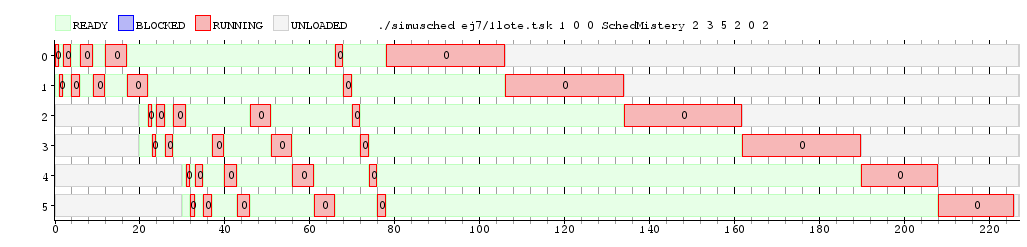
\includegraphics[width=1\textwidth]{../ej7/taskCpuMistery.png}
    \caption{Scheduler Mistery}
    %~ \label{fig:ej2_1nucleo}
\end{figure}


El costo de cambio de contexto y costa de migración de núcleo se decidió mantenerlo en 0, ya que no afecta el comportamiento del scheduler.
En el gráfico (nombre del grafico) se ve que las tareas se encolaron en la primera $colaReady$, ejecutan durante un solo tick y luego se encolan en 
la cola siguiente, que es la que tiene un quantum asociado igual a 2. El comportamiento sigue hasta que en el instante 20 llegan dos tareas nuevas.
Cuando la tarea 1 termina su quantum (instante 23), se empiezan a ejecutar las tareas en las colas con mayor prioridad, es decir 
las que acaban de llegar. Lo mismo sucede cuando llegan las tareas 4 y 5 en el el ciclo 30 de la simulación. Notar que las tareas 0 y 1 no vuelven
a obtener uso del cpu hasta el tick número 66. Esto es porque el scheduler le da prioridad a las tareas mas nuevas, ya que se encolan en las colas con
mayor prioridad. Esta característica podría hacer que las tareas mas "viejas" tarden demasiado tiempo en obtener el cpu si continuamente estan llegando 
nuaves tareas al sistema. 
Otra característica a observar es que efectivamente cuando se le asigna una tarea a la cola con quantum asociado 0, esta va a correr hasta hacer EXIT.

Para poder estudiar con mayor facilidad el comportamiento del scheduler cuando una tarea se bloquea, se creó dos tareas $Task1$ y $Task2$, que no reciben ningún
parámetro, hacen uso de cpu y realizan llamadas bloqueantes. 

El lote de tareas es:

\begin{itemize}

\item Task2BLOCK
\item Task1BLOCK
\item @15:
	TaskCPU 20

\end{itemize}

\begin{figure}[H]
  \centering
    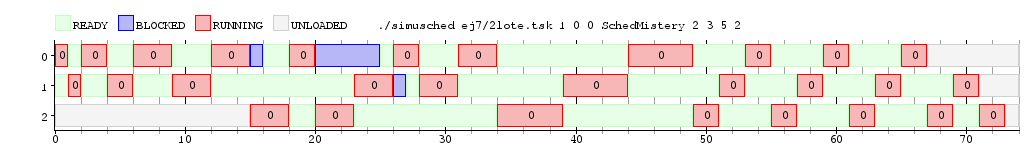
\includegraphics[width=1\textwidth]{../ej7/todojuntomistery.png}
    \caption{Scheduler Mistery}
    %~ \label{fig:ej2_1nucleo}
\end{figure}


En el instante 0 llegan dos tareas. La tarea 0 es $Task2BLOCK$ y la tarea 2 es $Task1BLOCK$. En el ciclo de clock número 15 llega la $TaskCPU$ y
las dos primeras tareas ya ejecutaron el quantum correspondiente a las tres primeras colas. En el instante 12, la tarea 0 se encuentra en la cola de con 
cantidad de quantum asociado 5. Pero en el ciclo 14 realiza una llamada bloqueante por lo que el scheduler la desaloja, y pasa a ejecutar a la tarea 2 que fue la 
última en llegar al sistema. Notar que como no hay ninguna otra tarea en las colas con quantum 1 y 2, solo la tarea 2 hace uso exclusivo del cpu 
del momento 15 al 18. Pero como al bloquearse una tarea, el scheduler la encola en la cola anterior a la que estaba, ahora pasa a ejecutar la tarea 0 nuevamente.
De nuevo realiza otra llamada bloqueante, por lo que ahora esta tarea va a pasar a la cola con quantum 2. Esto lo podemos observar en el instante 26, la tarea 0 
se ejecuta dos ciclos de clock. despues una vez que vuelve a hacer uso del cpu, realiza 3 ciclos y por ultimo pasa a la cola de quantum 5 y luego quantum 2 hasta que finaliza.
La tarea 1 también se realiza una llamada bloqueante en el tick número 25 en el momento que estaba en la cola de quantum 5. Se puede ver que la siguiente vez que 
ejecuta, se le asigna 3 ciclos de clock, que era lo esperado. 






% -------------------------------------------------------
% Ejercicio 8
% -------------------------------------------------------
%\newpage
%\subsection{Ejercicio 8}

En el ejercicio 8 se pide realizar una implementación del scheduler round robin, pero sin migración de procesos entre núcleos.
Para esto se agregaron nuevas estructuras a la clase SchedRR2:
colaReady: ahora es un vector de colas, las cuales van a almacenar los pid de las tareas que ultilicen el core correspondiente.
cantTasks: indica la cantidad de tareas que tiene cada cpu (RUNNING + BLOCKED + READY).
cpuTareasBloqueadas: es una cola de tuplas con un pid en la primera coordenada (proceso que hizo llamada bloqueante) y número de core en el cual estaba ejecutando.

Los métodos load, unblock y tick también cambian respecto del round robin con migración de procesos.
load(pid): ahora se encarga primero de buscar cual es el cpu con menor cantidad de tareas y, una vez encontrado, sumar uno a la cantTasks de ese cpu. Luego encola la tarea en la cola correspondiente de tareas ready.
unblock(pid): como se pide que no haya migración de procesos entre núcleos, se guarda en la estructura $cpuTareasBloqueadas$ todos las tareas bloqueadas con su número de 
core. Esta función encuentra la tupla en la cola, la quita de la cola, y luego encola la tarea en la colaReady del cpu obtenido.
tick(cpu, m): 
Motivo TICK sigue siendo similar a la implementación anterior.
Motivo BLOCK ademas de quitar al pid de la $colaReady$ del cpu, arma una tupla de la forma (pid, cpu), siendo pid = current_pid(cpu). Luego encola esa tupla en $cpuTareasBloqueadas$, 
si quedan tareas en la $colaReady$ toma la primera y devuelve su pid, y sino hay mas ready, devuelve IDLE_TASK.
Motivo EXIT acá se resta uno a la cantTasks del cpu actual, y se devuelve la tarea que sigue en la $colaReady$ y si no hay mas, IDLE_TASK.

Para corroborar su correcto funcionamiento se ideó un lote de tareas que permita chequear que, efectivamente no haya migración de núcleos y que se asignen correctamente 
los cores que cada tarea va a utilizar. 

Lote utilizado:

TaskCPU 20		
TaskConsola 20	1 5	
TaskCPU 5
@2: 
*2 TaskCPU 20
TaskCPU 5
@3:
TaskCPU 20
TaskConsola 10 1 5
TaskConsola 2 1 2
@18:				
TaskCPU 5
TaskConsola 3 2 4

La simulación se hizo con 3 cores con cambio de contexto 0, ya que no modifica el comportamiento del scheduler y costo de migración de núcleo 0.
La idea del lote, es cargar los primeros cores con tareas que tarden mas en terminar, y dejar en el ultimo tareas que vayan terminando y que liberen el cpu, 
para poder apreciar de esta forma, que efectivamente se asignará el cpu con menos tareas.
Debido a la implementación cuando todos los cores tengan igual cantidad de procesos, se le asignará el cpu mas chico numéricamente. 

GRAFICO

Se puede observar que no existe migración de núcleos, ya que todas las tareas mantienen su número de cpu a lo largo de toda la simulación.











% -------------------------------------------------------
% Ejercicio 9
% -------------------------------------------------------
%\input{ej9/ej9.tex}

% -------------------------------------------------------
% Ejercicio 10
% -------------------------------------------------------
%\input{ej10/ej10.tex}

\newpage
\bibliographystyle{plain}
\bibliography{tp3}

\end{document}

